%% Time-stamp: <2019-01-22 14:47:04 (marc)>
\documentclass[xcolor=x11names,compress,mathserif]{beamer}
\newcommand\hmmax{0}
\newcommand\bmmax{0}

\usepackage{../includes/MarkMathCmds}

\newcommand{\hackspace}{\hspace{4.2mm}}
\newcommand{\showstudent}[1]{}



% talk/author information
\newcommand{\authorname}{Mark van der Wilk}
\newcommand{\authoremail}{m.vdwilk@imperial.ac.uk}
\newcommand{\authoraffiliation}{
 Department of Computing\\Imperial
  College London}
\newcommand{\authortwitter}{markvanderwilk}
\newcommand{\slidesettitle}{\imperialBlue{Bayesian Optimisation}}
\newcommand{\footertitle}{Bayesian Optimisation}
\newcommand{\location}{Imperial College London}
\newcommand{\talkDate}{{February 17, 2022}}




\date{\imperialGray{\talkDate}}




% load defaults
\input{../includes/header.tex}
\input{../includes/titlepage.tex}





\begin{frame}{Optimisation of expensive cost functions}
In many situations, we want to optimise processes that we do not understand. They may be:
\begin{itemize}
\item Take long or costly to evaluate \\
  (physical experiments, or long-running computer simulations)
\item Black-box \\
  (we have little a-priori knowledge about them)
\item Impossible to evaluate gradients of \\
  (can't back-propagate through reality)
\end{itemize}
\end{frame}


\begin{frame}{Black-box cost functions}
  \begin{itemize}
  \item Design of turbine blades
  \item Biological molecules
  \item Optimise chemical processes
  \item \emph{Selecting Machine Learning hyperparameters}
  \end{itemize}

\begin{figure}
\centering
\includegraphics[width = 0.6\hsize]{./figures/bayesopt/Turbine-Blade}
\end{figure}

\end{frame}



\begin{frame}
\frametitle{Machine Learning Meta-Challenges}

\begin{itemize}
\item Machine learning models are getting more and more complicated
\\
\arrow Usually more parameters (e.g., deep neural networks)
\item Non-convex and stochastic optimization methods have
  meta-parameters that are difficult to tune (learning rates, momentum
  parameters, ...)
\end{itemize}
  \arrow Generally hard to apply modern techniques or reproduce
   results
\pause
\begin{myblock}{}
  Goal: Automate the selection of critical meta-parameters \\(see also:
  \cemph{Automated Machine Learning (AutoML)})
\end{myblock}
\end{frame}


%%%%%%%%%%%%%%%%%%%%%%%%%%%%%%%%%%%%%%%%%%%%%%%%%%%%%

\begin{frame}
\frametitle{Example: Deep Neural Networks}
\begin{figure}
\centering
\includegraphics[width = 0.3\hsize]{./figures/bayesopt/nn_art}
\hfill
\includegraphics[width=0.65\hsize]{./figures/bayesopt/DCNN_model}
\end{figure}

Huge interest in large neural networks
\begin{itemize}
\item When well-tuned, very successful for visual object
identification, speech recognition, computational biology, ...
\item Huge investments by Google, Facebook, Microsoft, etc.
\item \calert{Many choices:} number of layers, weight regularization,
layer size, which nonlinearity, batch size, learning rate
schedule, stopping conditions
\end{itemize}
\end{frame}


\begin{frame}
\frametitle{Example: Online Latent Dirichlet Allocation}


\begin{figure}
\centering
\includegraphics[height = 3cm]{./figures/bayesopt/lda}
\hfill
\includegraphics[height = 3cm]{./figures/bayesopt/gm_lda}
\end{figure}

\begin{itemize}
\item Hoffman et al. (2010): Approximate inference for \cemph{large-scale
  text analysis (topic modeling) with Latent Dirichlet Allocation}
\item Good empirical results when well tuned
\item \calert{Hyper-parameters} tricky to set: Dirichlet parameters, number of
  topics, learning rate schedule, batch size, vocabulary size, ...\nocite{Hoffman2010}
\end{itemize}
\end{frame}


\begin{frame}
\frametitle{Example: Classification of DNA Sequences}
\begin{figure}
\centering
\includegraphics[height = 3cm]{./figures/bayesopt/SVM}
\hspace{5mm}
\includegraphics[height = 3cm]{./figures/bayesopt/protein}
\end{figure}

\begin{itemize}
\item Objective: Predict which DNA sequences will bind with which
  proteins
\item Miller et al. (2012):\nocite{Miller2012} \cemph{Latent Structural
  Support Vector Machine}
\item \calert{Hyper-parameters:} margin/slack parameter, entropy parameter,
  convergence criterion
\end{itemize}
\end{frame}




\begin{frame}
\frametitle{Search for Good Hyper-parameters}

\begin{itemize}
\item Define an objective function to evaluate the quality of the hyper-parameters
\begin{itemize}
\item Usually, we care about generalization performance
\item Cross validation to measure parameter quality
\end{itemize}
\pause
\item Standard search procedures:
\begin{itemize}
\item Manual tuning
\item Grid search
\item Random search (very simple, works surprisingly well)
\item Black magic
\end{itemize}
\pause
\item Painful:
\begin{itemize}
\item Evaluating the quality of the objective may be very expensive
  (e.g., time or money)\\
  \arrow Imagine we would need to run a GPU/TPU cluster for 2 weeks
\item Many training cycles
\item Possibly noisy
\end{itemize}
\end{itemize}
\end{frame}




\begin{frame}
\frametitle{Alternative Approach: Bayesian Optimization}
\begin{myblock}{Setting}
Globally optimize a black-box objective that is expensive to evaluate
(e.g., cross-validation error for a massive neural network)
\end{myblock}

We want to be smart about using the evaluations we have
\pause
\begin{itemize}[<+->]
\item Build a \cemph{probabilistic proxy model} for the objective using
  outcomes of past experiments as training data
\item We can predict the outcome of the next experiment using the proxy model, which is much \cemph{cheaper to evaluate}
%\item Use posterior predictive distribution of the probabilistic model
\item \cemph{Optimize cheap proxy} function to determine where to evaluate the true
  objective next
\item Standard proxy: \cemph{Gaussian process}
\end{itemize}
% \begin{myblock}{}
% The main insight:
% Make the proxy function exploit uncertainty to balance
% exploration against exploitation.

% \end{myblock}
\end{frame}

%%%%%%%%%%%%%%%%%%%%%%%%%%%%%%%%%%%%%%%%%%%%%%%%%%%%%

\begin{frame}
\frametitle{Setting (2)}
\begin{itemize}
\item Objective: Find global minimum of objective function $f$:
 $$\vec x_* = \arg\min_{\vec x} f(\vec x)$$
\item We can evaluate the objective $g$ pointwise, but do not have an easy
  functional form or gradients; observations may be noisy
\item \calert{Evaluating $f$ is costly} (e.g., train a massive deep network)
\end{itemize}

\begin{figure}
\centering
\includegraphics[height = 4cm]{./figures/bayesopt/bo_init}
\end{figure}
\end{frame}






% \begin{frame}{Recap: Prospecting for gold}
% First choose location to prospect at $p$,
% then choose location to mine $m$. \pause
% \begin{enumerate}[{\hspace{0.3cm}Step} 1:]
% \item $U(\vx, d_p, m, p) = -c_p + x_m$ \pause
% \item $\Exp{p(\vx, d_p)}{U(\vx, d_p, m, p)} = \Exp{p(\vx, d_p)}{-c_p + x_m}$ \pause
% \item $\text{action} = \argmax_{\text{actions}} \Exp{p(\vx, d_p)}{U(\vx, d_p, m, p)}$ \end{enumerate}

% % \begin{align}
% % U(\vx, d_p, m, p) &= -c_p + x_m \\
% % \Exp{p(\vx, d_p)}{U(\vx, d_p, m, p)} &= \Exp{p(\vx, d_p)}{-c_p + x_m} \\
% % \end{align}
% \pause
% \vspace{0.4cm}
% Trick is to realise that
% \begin{align}
% m(d_p) = \argmax_n \Exp{p(\vx\given d_p)}{x_n} = \argmax_n \mu_n'(d_p)
% \end{align}
% \pause
% so...
% \begin{align}
% U(\vx, d_p, p) &= -c_p + x_{m(d_p)} \\
% \Exp{p(\vx, d_p)}{U(\vx, d_p, p)} &= -c_p + \Exp{p(d_p)}{\Exp{p(\vx\given d_p)}{x_{m(d_p)}}} \\
% &= -c_p + \Exp{p(d_p)}{\max_{n}\mu_n'}
% \end{align}
% \end{frame}


\begin{frame}{Bayesian optimisation}
Let's phrase BayesOpt using decision theory:
\begin{align}
L(f, \{\vx_n\}_{n=1}^N) = Nc + \min_{1 \leq n \leq N} f(\vx_n)
\end{align}
(Optimisers are pessimists, they talk about loss instead of utility)
\pause
\begin{itemize}
\item We decide how many evaluations we want to do $N$
\item We decide where to evaluate $f(\cdot)$
\item We incur a cost $c$ for each evaluation
\item We reduce loss by finding a lower $f(\vx)$
\end{itemize}
\end{frame}


\begin{frame}{Bayesian optimisation -- decision theory}
For 3 observations:
\begin{align}
\{\vx_1^*, \vx_2^*(\data_1), \vx_3^*(\data_2)\} = \argmin_{\{\vx_n\}_{n=1}^3} \Exp{p(f)}{Nc + \min_{1\leq n\leq N} f(\vx_n)}
\end{align}
\pause
Remember: actions $\vx_2$ and $\vx_3$ can depend on the data we observe. The data are observations of the GP $\data = \{\vx_n, f(\vx_n)\}_{n=1}^N$.
\pause
\begin{align}
\vx_1^* = -Nc + \argmin_{\vx_1} \Exp{f}{\min_{\vx_2} \Exp{f\given \data_1}{\min_{\vx_3} \Exp{f\given \data_2}{\min_{1 \leq n \leq 3} \{f(\vx_n)\}}}}
\end{align}
\end{frame}


\begin{frame}{Computational difficulties}
\begin{align*}
\vx_1^* = -Nc + \argmin_{\vx_1} \Exp{f}{\min_{\vx_2} \Exp{f\given \data_1}{\min_{\vx_3} \Exp{f\given \data_2}{\min_{1 \leq n \leq 3} \{f(\vx_n)\}}}}
\end{align*}

\vspace{0.3cm}

\pause

This is \emph{very} difficult to evaluate.
\begin{itemize}
\item Difficult optimisations: closed-form optimum cannot be found
\item Expectations of non-closed-form expressions
\item Optimisations of expectations of non-closed-form expressions
\end{itemize}

\vspace{0.4cm} \pause

Alternative approaches:
\begin{itemize}
\item Can try to approximate these quantities (fun to try for small-scale examples)
\item Heuristic approaches
\end{itemize}
\end{frame}



\begin{frame}{How to design a heuristic}
In BayesOpt, heuristic is called the \emph{acquisition function}. Instead of maximising the utility (or minimising loss), we maximise the acquisition function.
\pause
\begin{itemize}
\item Computational constraint: Only use posterior of GP given \emph{current} observations to choose current action \pause
\item Desired behaviour: Some sort of a trade-off between \emph{exploration} and \emph{exploitation}. \pause
\begin{itemize}
\item Want to try inputs that are different (exploration)
\item Want to focus on areas that are likely to have high values (exploitation)
\end{itemize}
\end{itemize}
\end{frame}

% \begin{itemize}
% \item Computational constraint: Only use posterior of GP given \emph{current} observations
% \item Desired behaviour: Some sort of a trade-off between \emph{exploration} and \emph{exploitation}.
% \end{itemize}
% posteiror of


\begin{frame}{Inadequate acquisition functions}
Two inadequate acquisition functions:
\begin{itemize}
  \item Minimise posterior mean (pure exploitation)
  \item Maximise posterior variance (pure exploration)
\end{itemize}
\begin{figure}
\includegraphics[height = 5cm]{./figures/bayesopt/BOa3}
\end{figure}
\end{frame}



\begin{frame}
  \frametitle{Common acquisition functions}

\begin{itemize}
\item For all $\vec x\in\R^D$ the GP posterior gives a predictive mean
  $\mu(\vec x)$ variance $\sigma^2(\vec x)$ of $g(\vec x)$
\item Define
$$
\green{\gamma(\vec x) = \frac{f(\vec x_{\text{best}}) - \mu(\vec
  x)}{\sigma(\vec x)}}
$$
\pause
\item  \emph{Probability of Improvement (Kushner 1964)\nocite{Kushner1964}:}
$$
\alpha_{\text{PI}}(\vec x) = \Phi(\green{\gamma(\vec x)})
$$
\item \emph{Expected Improvement (Mockus 1978)\nocite{Mockus1978}:}
$$
\alpha_{\text{EI}}(\vec x) = \sigma(\vec x)\big(\green{\gamma (\vec x)}\Phi(\green{\gamma(\vec
x)}) + \gaussx{\green{\gamma(\vec x)}}{0}{1}\big)
$$
\item \emph{GP Lower Confidence Bound (Srinivas et al., 2010):\nocite{Srinivas2010}}
$$
\alpha_{\text{LCB}}(\vec x) = - (\mu(\vec x) - \kappa\sigma(\vec
x))\,,\quad\kappa > 0
$$
\end{itemize}
\end{frame}






\begin{frame}
\frametitle{Probability of Improvement (1)}
\begin{columns}
\column{0.5\hsize}
\begin{figure}
\centering
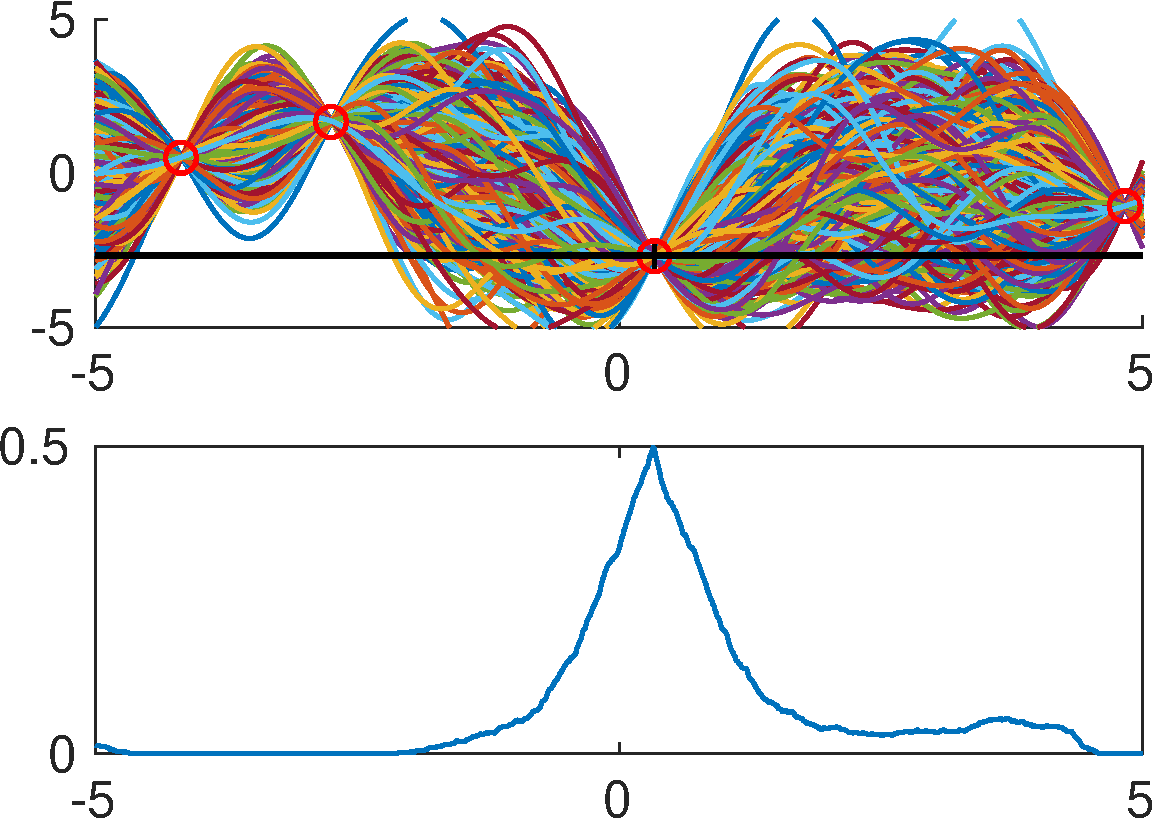
\includegraphics[width = \hsize]{./figures/bayesopt/bo_PI_samples_no_slack}
\end{figure}
\column{0.5\hsize}
\begin{itemize}
\item \cemph{Idea:} Determine the probability that $\vec x_*$ leads to a better
  function value than the currently best one $f(\vec x_{\text{best}})$
\item Sampling-based setting: Sample $N$ functions $f_i$; at every
  input $\vec x$ compute a Monte-Carlo estimate
\end{itemize}
\end{columns}

\begin{align*}\alpha_{\text{PI}}(\vec x) &= p(f(\vec x) < f(\vec
 x_{\text{best}}))\approx \frac{1}{N}\sum\nolimits_{i=1}^N \delta\big(f_i(\vec x) <
  f(\vec x_{\text{best}})\big)
 \end{align*}
\pause
\arrow Can lead to continued exploitation in an $\epsilon$-region around $\vec
x_{\text{best}}$.\\
\pause
\arrow Introduce a ``slack variable'' $\xi$ for more aggressive exploration
\end{frame}

%%%%%%%%%%%%%%%%%%%%%%%%%%%%%%%%%%%%%%%%%%%%%%%%%%%%%
\begin{frame}
\frametitle{Probability of Improvement (2)}
\begin{figure}
\centering
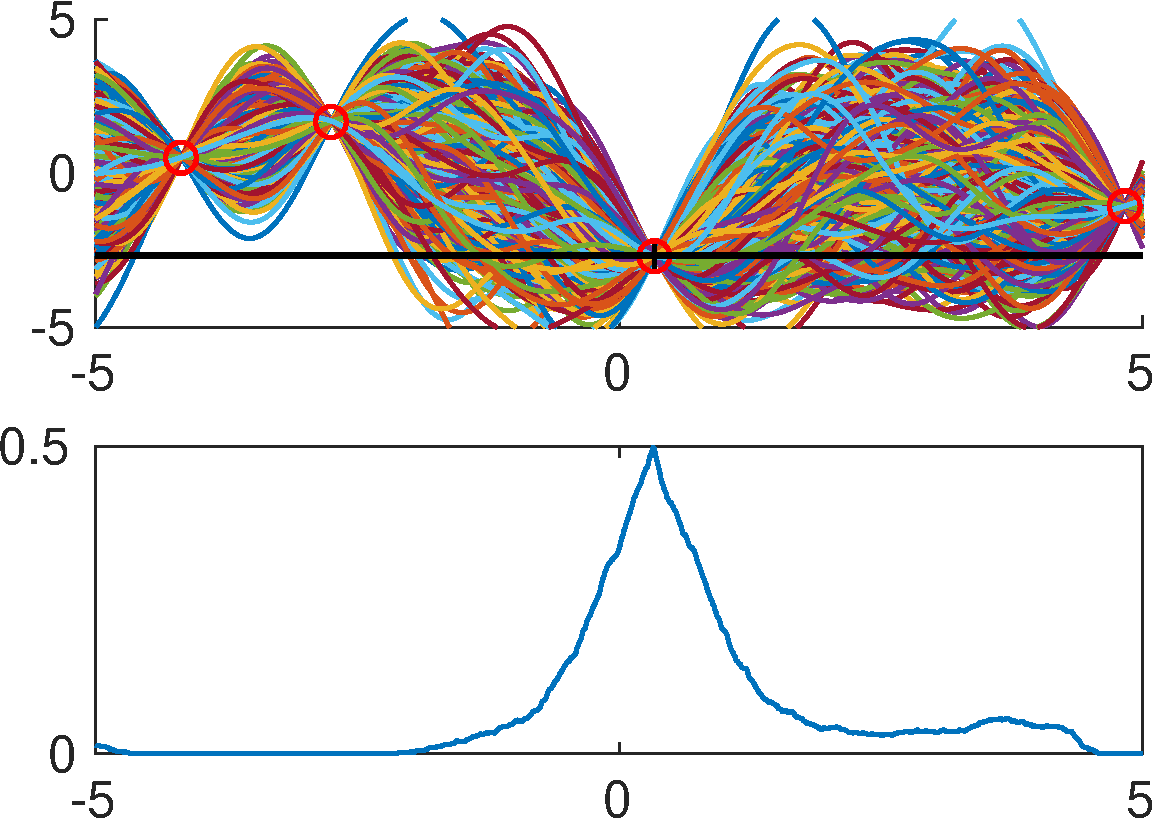
\includegraphics[width = 0.48\hsize]{./figures/bayesopt/bo_PI_samples_no_slack}
\hfill
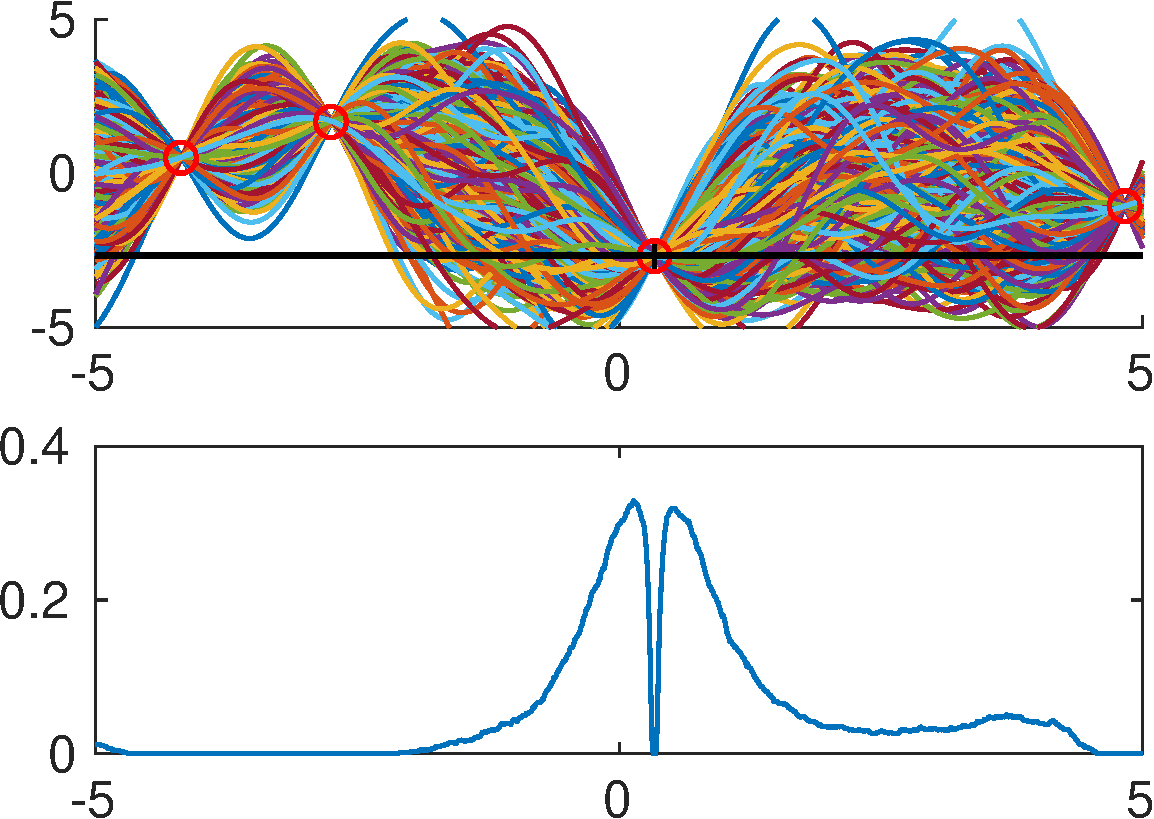
\includegraphics[width = 0.48\hsize]{./figures/bayesopt/bo_PI_samples_with_slack}
\end{figure}
\vspace{-5mm}
\begin{itemize}
\item Look at a minimum improvement of $\colchar{$\xi$}{blue}>0$:
 $$\alpha_{\text{PI}}(\vec x) = p(f(\vec x) < f(\vec x_{\text{best}})\colchar{$-\xi$}{blue}) \approx \frac{1}{N}\sum\nolimits_{i=1}^N \delta\big(f_i(\vec x) < f(\vec x_{\text{best}})\colchar{$-\xi$}{blue}\big)$$
\item If $f\sim GP$ and $p(f(\vec x)) = \gauss{\mu(\vec
    x)}{\sigma(\vec x)}$:
\begin{align*}
\alpha_{\text{PI}}(\vec x) =  \Phi(\gamma(\vec x, \xi))\,,\qquad
\gamma(\vec x, \xi) = \frac{f(\vec x_{\text{best}}) \colchar{$- \xi$}{blue} - \mu(\vec
  x)}{\sigma(\vec x)}
\end{align*}
\end{itemize}


\end{frame}
%%%%%%%%%%%%%%%%%%%%%%%%%%%%%%%%%%%%%%%%%%%%%%%%%%%%%
%\input{pi_example}
%%%%%%%%%%%%%%%%%%%%%%%%%%%%%%%%%%%%%%%%%%%%%%%%%%%%%

\begin{frame}
\frametitle{Expected Improvement}
\begin{columns}

\column{0.5\hsize}
\begin{itemize}
\item \cemph{Idea:} Quantify the \cemph{amount of improvement}
\item Sampling-based scenario, where $f_i\sim p(f)$:
\begin{align*}
\alpha_{\text{EI}}(\vec x) = \E[ \max\{0, f(\vec x_{\text{best}}) - f(\vec
x)\}] \\
\approx \frac{1}{N} \sum_{i=1}^N \max \{0, f(\vec x_{\text{best}}) -  f_i(\vec x) \}
\end{align*}
\end{itemize}
\column{0.45\hsize}
\begin{figure}
\centering
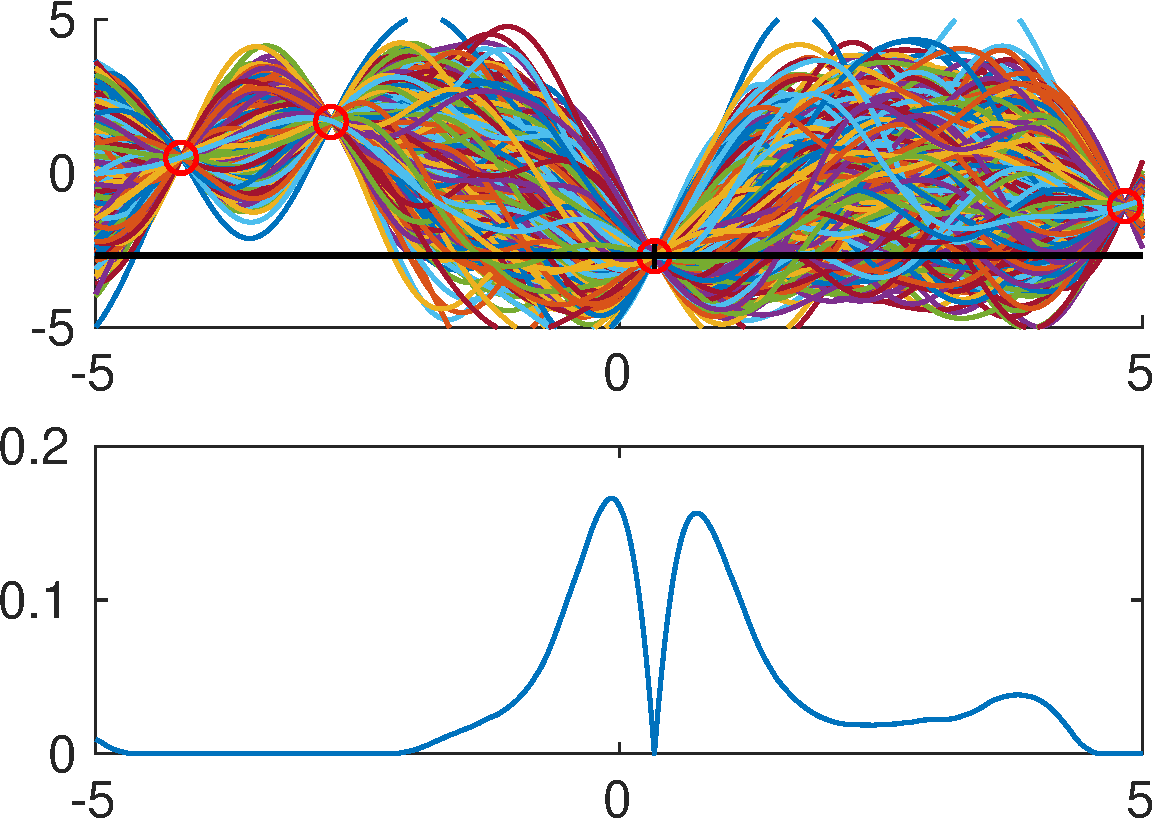
\includegraphics[width = \hsize]{./figures/bayesopt/bo_EI_samples}
\end{figure}
\end{columns}

\begin{itemize}
\item If $f\sim GP$, we have a closed-form expression:
\begin{align*}
\alpha_{\text{EI}}(\vec x) = \sigma(\vec x)\big(\gamma (\vec x)\Phi(\gamma(\vec
x)) + \gaussx{\gamma(\vec x)}{0}{1}\big)
\end{align*}
\item Slack-variable approach also possible (similar to PI)~\nocite{Lizotte2008,Brochu2009}
\end{itemize}
\end{frame}

%%%%%%%%%%%%%%%%%%%%%%%%%%%%%%%%%%%%%%%%%%%%%%%%%%%%%

\begin{frame}
\frametitle{GP-Lower Confidence Bound (1)}
\begin{figure}
\centering
\includegraphics[height = 4cm]{./figures/bayesopt/bo_example_ucb}
\end{figure}
\begin{itemize}
\item Use the predictive mean $\mu(\vec x) $ and variance
  $\sigma^2(\vec x)$ of the GP prediction directly for
  targeted exploration by means of the acquisition function
\begin{align*}
\alpha_{\text{LCB}}(\vec x_t) = -\big( \mu(\vec x_t) - \sqrt{\kappa}\sigma(\vec x_t)\big)
\end{align*}
% In practice: Use
% $\max \{0, g(\vec x_{\text{best}}) - \alpha_{\text{LCB}}(\vec x_t) \}$
%max(fbest_LCB - UCB(-kappa, post_mean_LCB, sqrt(post_var_LCB)),0);

\end{itemize}
\end{frame}

%%%%%%%%%%%%%%%%%%%%%%%%%%%%%%%%%%%%%%%%%%%%%%%%%%%%%

\begin{frame}
\frametitle{GP-Lower Confidence Bound (2)}
\begin{figure}
\centering
\includegraphics[height = 4cm]{./figures/bayesopt/bo_example_ucb}
\end{figure}
\begin{itemize}
\item More generally, we can get regret bounds for iteration-dependent
  $\kappa$ (Srinivas et al., 2010)\nocite{Srinivas2010}
\begin{align*}
  \alpha_{\text{LCB}}(\vec x_t) = -\big(\mu(\vec x_{t}) - \sqrt{\kappa_t}\sigma(\vec x_{t})\big)
\end{align*}
where $\kappa_t\in\mathcal O(\log t)$ grows with the iteration $t$
\\
\arrow Continue exploration
\end{itemize}
\end{frame}





\begin{frame}
\frametitle{Bayesian Optimization: Illustration}


\onslide*<1>{
\begin{figure}
\includegraphics[height = 5cm]{./figures/bayesopt/BOa1}\hspace{1.2mm}
\end{figure}
}
\onslide*<2>{
\begin{figure}
\includegraphics[height = 5cm]{./figures/bayesopt/BOb1}\hspace{1.2mm}
\end{figure}
}
\onslide*<3>{
\begin{figure}
\includegraphics[height = 5cm]{./figures/bayesopt/BOa2}\hspace{1.2mm}
\end{figure}
}
\onslide*<4>{
\begin{figure}
\includegraphics[height = 5cm]{./figures/bayesopt/BOb2}\hspace{1.2mm}
\end{figure}
}
\onslide*<5>{
\begin{figure}
\includegraphics[height = 5cm]{./figures/bayesopt/BOa3}
\end{figure}
}
\onslide*<6>{
\begin{figure}
\includegraphics[height = 5cm]{./figures/bayesopt/BOb3}
\end{figure}
}
\onslide*<7>{
\begin{figure}
\includegraphics[height = 5cm]{./figures/bayesopt/BOa4}
\end{figure}
}
\onslide*<8>{
\begin{figure}
\includegraphics[height = 5cm]{./figures/bayesopt/BOb4}
\end{figure}
}
\onslide*<9>{
\begin{figure}
\includegraphics[height = 5cm]{./figures/bayesopt/BOa5}
\end{figure}
}
\onslide*<10>{
\begin{figure}
\includegraphics[height = 5cm]{./figures/bayesopt/BOb5}
\end{figure}
}
\onslide*<11>{
\begin{figure}
\includegraphics[height = 5cm]{./figures/bayesopt/BOa6}
\end{figure}
}
\onslide*<12>{
\begin{figure}
\includegraphics[height = 5cm]{./figures/bayesopt/BOb6}
\end{figure}
}
\onslide*<13>{
\begin{figure}
\includegraphics[height = 5cm]{./figures/bayesopt/BOa7}
\end{figure}
}
\onslide*<14>{
\begin{figure}
\includegraphics[height = 5cm]{./figures/bayesopt/BOb7}
\end{figure}
}
\onslide*<15>{
\begin{figure}
\includegraphics[height = 5cm]{./figures/bayesopt/BOa8}
\end{figure}
}
\onslide*<16>{
\begin{figure}
\includegraphics[height = 5cm]{./figures/bayesopt/BOb8}
\end{figure}
}
\onslide*<17>{
\begin{figure}
\includegraphics[height = 5cm]{./figures/bayesopt/BOa9}
\end{figure}
}
\onslide*<18>{
\begin{figure}
\includegraphics[height = 5cm]{./figures/bayesopt/BOb9}
\end{figure}
}
\onslide*<19>{
\begin{figure}
\includegraphics[height = 5cm]{./figures/bayesopt/BOa10}
\end{figure}
}
\onslide*<20>{
\begin{figure}
\includegraphics[height = 5cm]{./figures/bayesopt/BOb10}
\end{figure}
}
\onslide*<21>{
\begin{figure}
\includegraphics[height = 5cm]{./figures/bayesopt/BOa11}
\end{figure}
}
\onslide*<22>{
\begin{figure}
\includegraphics[height = 5cm]{./figures/bayesopt/BOb11}
\end{figure}
}
%
%
% \begin{itemize}
% \item \cemph{Lower-Confidence-Bound} (LCB) criterion to select next point
% $$
% \theta^* \in \arg\min_{\theta} \quad\E[\tilde g(\theta)] -
% 2\sqrt{\var[\tilde g(\theta)]}
% $$
% %\onslide+<22->{
% \only<22>{\item Global minimum found after 10 function evaluations}
% %}
% \phantom{1}
% \end{itemize}


\end{frame}









%%%%%%%%%%%%%%%%%%%%%%%%%%%%%%%%%%%%%%%%%%%%%%%%%%%%%

\begin{frame}
\frametitle{Optimising the Acquisition Function}
Notice: Acquisition function is multi-modal \pause
\begin{itemize}
\item Optimizing the acquisition function \calert{requires us to run a global
  optimizer inside Bayesian optimization}
\item What have we gained?
\pause
\item Evaluating the acquisition function is cheap compared to
  evaluating the true objective\\
\arrow We can afford evaluating it many times \\
\arrow Apply the usual tricks of many random restarts
\end{itemize}

% \begin{figure}
%   \centering
% \includegraphics[height = 2.1cm]{./figures/bayesopt/netflix}
% \hspace{5mm}
% \includegraphics[height = 2.1cm]{./figures/bayesopt/oil}
% \hspace{5mm}
% \includegraphics[height = 2.1cm]{./figures/bayesopt/alphago}\nocite{Chen2018}
% \end{figure}

\end{frame}



\begin{frame}
\frametitle{Key Steps (Pseudo-Code)}
\begin{algorithmic}[1]
\State \textbf{Init:} Data set $\mathcal D_0 = \{\mat X_0, \vec y_0\}$ (can be empty)
\For {iterations $t=1, 2, ...$}
\State \cemph{Update GP} using data $\mathcal D_{t-1}$
\State Select $\vec x_{t} = \arg\max_{\vec x} \alpha(\vec x)$ by
\cemph{optimising acquisition function}
\State Query true objective $g$ at $\vec x_{t}$
\State Augment data set $\mathcal D_{t} = \mathcal D_{t-1} \cup \{(\vec
x_{t}, y_{t})\}$
\EndFor
\State \textbf{Return} best input in data set: $\vec x^* = \arg\min_{\vec x} y(\vec x)$
\end{algorithmic}

Optimising acquisition function is itself an iterative process, done with a numerical gradient-based optimiser (e.g.~BFGS).
\end{frame}



\begin{frame}
\frametitle{Limitations}
\begin{itemize}
\item Getting the function model (e.g., covariance function) wrong can
  be catastrophic \pause
\begin{itemize}
\item Model will not correctly predict where function is high
\item Over/under estimation of uncertainty will lead to over/under exploration
\end{itemize}
\pause
\item Limited scalability in the number of dimensions and/or
  evaluations of the true
  objective function\\ \pause
\begin{itemize}
\item Local kernels too uncertain in high dimensions
\item Gaussian processes expensive for large datasets \pause (although BayesOpt generally doesn't have the problem of large datasets...)
\end{itemize}
\end{itemize}
\end{frame}

%%%%%%%%%%%%%%%%%%%%%%%%%%%%%%%%%%%%%%%%%%%%%%%%%%%%%
\begin{frame}
\frametitle{Poor Model Choice}
\begin{figure}
\centering
\includegraphics[width = 0.48\hsize]{./figures/bayesopt/samplesGauss}
\includegraphics[width = 0.48\hsize]{./figures/bayesopt/samplesMatern3}
\end{figure}

\begin{itemize}
\item Covariance function selection is crucial for good performance\\
\arrow Choose a sufficiently flexible and adaptive kernel, e.g.,
Mat\'ern (but not the squared exponential (Gaussian))
\pause
\item Nice side-effect of Mat\'ern: Exploration is more encouraged than with
  the Gaussian kernel
\end{itemize}

\end{frame}
%%%%%%%%%%%%%%%%%%%%%%%%%%%%%%%%%%%%%%%%%%%%%%%%%%%%%
\begin{frame}
\frametitle{Choosing Covariance Functions}
Application:
\begin{itemize}
\item Structured SVM for Protein Motif Finding (Miller et al.,
2012)\nocite{Miller2012}
\item  Optimize hyper-parameters of SSVM using
BO (Snoek et al., 2012)\nocite{Snoek2012}
\end{itemize}
\begin{figure}
\centering
\includegraphics[width = 0.68\hsize]{./figures/bayesopt/ssvmmotif_comparison_kernel}
\caption{Figure from Snoek et al. (2012)~\nocite{Snoek2012}}
\end{figure}



\end{frame}



%%%%%%%%%%%%%%%%%%%%%%%%%%%%%%%%%%%%%%%%%%%%%%%%%%%%%

\begin{frame}
\frametitle{Gaussian Process Hyper-Parameters}
\begin{itemize}[<+->]
\item \calert{Empirical Bayes (maximize the marginal likelihood) can fail
  horribly,} especially in the early stages of Bayesian optimization
  when we have only a few data points
\item Solution: Integrate out the GP hyper-parameters $\vec\theta$ by \cemph{Markov Chain
  Monte Carlo (MCMC)} sampling (e.g., slice sampling)
\item Look at \cemph{integrated acquisition function}
\begin{align*}
\alpha(\vec x) &= \E_{\vec \theta}[\alpha(\vec x, \vec\theta)] = \int \alpha(\vec x,\vec\theta)p(\vec\theta)
  d\vec\theta\\
&\approx \frac{1}{K}\sum_{k=1}^K \alpha(\vec
  x,\vec\theta^{(k)})\,,\quad \vec\theta^{(k)}\sim\hspace{-5mm}
  \underbrace{p(\vec\theta|\mat X_n, \vec y_n)}_{\text{hyper-parameter
  posterior}}
\end{align*}
\end{itemize}
\end{frame}
%%%%%%%%%%%%%%%%%%%%%%%%%%%%%%%%%%%%%%%%%%%%%%%%%%%%%
\begin{frame}
\frametitle{Integrating out GP Hyper-parameters}
\begin{itemize}
\item Online LDA (Hoffman et al., 2010)~\nocite{Hoffman2010} for topic
  modeling
\item Two critical hyper-parameters that control the learning rate
  learned by BO (Snoek et al., 2012) \nocite{Snoek2012}
\end{itemize}
\begin{figure}
\centering
\includegraphics[width = 0.68\hsize]{./figures/bayesopt/onlinelda_comparison}
\caption{Figure from Snoek et al. (2012)~\nocite{Snoek2012}}
\end{figure}

\end{frame}


%%%%%%%%%%%%%%%%%%%%%%%%%%%%%%%%%%%%%%%%%%%%%%%%%%%%%
\begin{frame}
\frametitle{Robots That Learn to Recover from Damage}
\begin{figure}
\includegraphics[width = 0.9\hsize]{./figures/bayesopt/robot_fix_learn}
\\
Cully et al. (2015)\nocite{Cully2015}
\end{figure}
\end{frame}


%%%%%%%%%%%%%%%%%%%%%%%%%%%%%%%%%%%%%%%%%%%%%%%%%%%%%

\begin{frame}
\frametitle{Application Example: Controller Learning in Robotics
  {\small (Calandra et al., 2015)}}
\begin{minipage}[t]{0.65\hsize}
\begin{itemize}
\item Fragile bipedal robot \\
\arrow Only few experiments feasible
\item Maximize robustness and walking speed
\item 4 motors: \\
2 actuated hips + 2 actuated knees
\item Controller implemented as a finite-state-machine (8 parameters)
\onslide+<2->{
\item Good parameters found after 80--100 experiments
\item \cemph{Substantial speed-up} compared to manual parameter search
}
\end{itemize}
\end{minipage}
\begin{minipage}[t]{0.3\hsize}
\begin{figure}
\centering
 \movie[externalviewer, poster]{\includegraphics[height =
  4.5cm]{./figures/bayesopt/fox}}{/home/marc/research/svn/marc/videos/fox_gait_optimization_summary_short.mpeg}
\\
{\small Calandra et al. (2015)\nocite{Calandra2015a}}
\end{figure}
\end{minipage}
%

\end{frame}
%%%%%%%%%%%%%%%%%%%%%%%%%%%%%%%%%%%%%%%%%%%%%%%%%%%%%
\begin{frame}
\frametitle{Comparison}
\begin{figure}
\centering
\includegraphics[height = 4cm]{./figures/bayesopt/fox_opt_curves}
\end{figure}


\begin{itemize}
\item Squared exponential covariance function
\item Learned GP hyper-parameters (no MCMC for integrating them out)
\end{itemize}

\end{frame}



% %%%%%%%%%%%%%%%%%%%%%%%%%%%%%%%%%%%%%%%%%%%%%%%%%%%%%
%
% \begin{frame}
% \frametitle{Applications}
% \nocite{Calandra2015a, Lizotte2008, Martinez-Cantin2007}
% \begin{itemize}
% \item Robotics
% \item Cheetah robot
% \item Training neural networks
% \item Optimizing simulators
% \item Wetlab and Twitter
% \end{itemize}
%
% \end{frame}
%%%%%%%%%%%%%%%%%%%%%%%%%%%%%%%%%%%%%%%%%%%%%%%%%%%%%
\begin{frame}
\frametitle{Further Topics in BO}

\begin{itemize}
\item \cemph{Entropy-based acquisition functions:} Directly describe the distribution over the best input location (Hennig \& Schuler, 2012; Hern\'andez-Lobato et al., 2014)
\item \cemph{Non-myopic} Bayesian optimization (e.g., Osborne et al., 2009)\nocite{Osborne2009}
\item \cemph{High-dimensional} optimization (e.g., Wang et al., 2016)\nocite{Wang2016}
\item \cemph{Large-scale} Bayesian optimization (Hutter et al., 2014)\nocite{Hutter2014}
\item \cemph{Efficient optimization of acquisition functions} (Wilson et al., 2018)\nocite{Wilson2018}
\item \cemph{Non-GP} Bayesian optimization (Hutter et al., 2014; Snoek et al.,
  2015)\nocite{Jones1998, Hutter2014,Snoek2015, Springenberg2016}
\item \cemph{Constraints} (e.g., Gelbart et al., 2014)\nocite{Gelbart2014}
\item \cemph{Automated machine learning} (e.g., Feurer et al.,
  2015)\nocite{Feurer2015}
\item \cemph{Multi-tasking, parallelizing, resource allocation}, ... (e.g.,
  Swersky et al., 2014; Snoek et al., 2012; Wilson et al., 2018)\nocite{Swersky2014, Snoek2012}

\end{itemize}



\end{frame}

%%%%%%%%%%%%%%%%%%%%%%%%%%%%%%%%%%%%%%%%%%%%%%%%%%%%%
\begin{frame}
\frametitle{Software}
\begin{itemize}
\item \cemph{BayesOpt} \url{https://bitbucket.org/rmcantin/bayesopt/}
  (Martinez-Cantin, 2014)\nocite{Martinez-Cantin2014}
\item \cemph{Spearmint} \url{https://github.com/HIPS/Spearmint}
\item \cemph{Pybo} \url{https://github.com/mwhoffman/pybo} (Hoffman \& Shariari)
\item \cemph{GPyOpt} \url{https://github.com/SheffieldML/GPyOpt}
  (Gonzalez et al.)
\item Matlab toolbox (bayesopt)
\end{itemize}
\end{frame}


%%%%%%%%%%%%%%%%%%%%%%%%%%%%%%%%%%%%%%%%%%%%%%%%%%%%%
\begin{frame}{Summary}

  \begin{figure}
    \centering
      \includegraphics[height=2.5cm]{./figures/bayesopt/protein}
  \hspace{5mm}
    \includegraphics[height = 2.5cm]{./figures/bayesopt/alphago}
    \hspace{5mm}
    \movie[externalviewer, poster]{\includegraphics[height =
  2.5cm]{./figures/bayesopt/fox}}{/home/marc/research/svn/marc/videos/fox_gait_optimization_summary_short.mpeg}
  \end{figure}
  
  
  \begin{itemize}
    \item Global optimization of black-box functions, which are
      expensive to evaluate
    %
      \arrow Meta-challenges in machine learning, Auto-ML
    \item Use a probabilistic proxy model that is cheap to evaluate
      and use this to suggest next experiments
    \item Acquisition function trades of exploration and exploitation
  \end{itemize}
  
\end{frame}









% \begin{frame}{Coursework}
% \begin{itemize}
% \item Part tutorial to guide you though a simple GP implementation
% \item Assessed part on Bayesian optimisation
% \item Submission through labts
% \item Will be released later today or tomorrow
% \item Full description on Piazza
% \end{itemize}
% \end{frame}


\begin{frame}{Further Reading}
  \begin{itemize}
  \item Brochu et al.: \textit{A Tutorial on Bayesian Optimization of
    Expensive Cost Functions, with Application to Active User Modeling
    and Hierarchical Reinforcement Learning}, arXiv:1012.2599, 2012
  \item Shahriari et al.: \textit{Taking the Human Out of the Loop: A Review
    of Bayesian Optimization}, Proceedings of the IEEE, 2016
  \end{itemize}
\end{frame}










%%%%%%%%%%%%%%%%%%%%%%%%%%%%%%%%%%%%%%%%%
% REFERENCES
%%%%%%%%%%%%%%%%%%%%%%%%%%%%%%%%%%%%%%%%%
\begin{frame}[t,allowframebreaks]
\frametitle{References}
\linespread{1.0}
\tiny
\bibliographystyle{abbrv}
\bibliography{../includes/pi-literature}
\end{frame}



\end{document}
%%% Local Variables: 
%%% mode: latex
%%% TeX-master: t
%%% End: 
